%*****************************************************************************%
% This LaTeX-Template is based on the beamer package:                         %
% http://latex-beamer.sourceforge.net                                         %
%                                                                             %
% For further details on how to create beamer slides you can check their      %
% documentation:                                                              %
% http://mirror.ctan.org/macros/latex/contrib/beamer/doc/beameruserguide.pdf  %
%                                                                             %
% The layout fits the current standard of the acg color scheme.               %
% Version: 1.0                                                                %
% Authors: Lars Krecklau <krecklau@informatik.rwth-aachen.de>                 %
%*****************************************************************************%
\documentclass{beamer}

\usepackage{graphicx}
\usepackage[german]{babel}

% Place in these lines your title and the author's names:
\newcommand{\myTitle}{Milestone 3 - Marble Race Game - Group C}
\newcommand{\myAutors}{Fabian Klemp, Steffen F\"undgens, Simon Froitzheim, Jasper Manousek}
\newcommand{\myAutorsFoot}{\myAutors}

% If you want to draw images by latex:
% http://www.texample.net/tikz/
\usepackage{tikz}
\usetikzlibrary{arrows,shapes}

% Apply the acg layout
\mode<presentation>
{
    \usetheme{Darmstadt}
    \useoutertheme{miniframes}
    \usecolortheme{acg}
    
    \setbeamercovered{transparent}
    \setbeamertemplate{navigation symbols}{}
    \setbeamertemplate{footline}
    {
        
\includegraphics[width=\paperwidth]{images/logo.png}
        \vspace*{-0.8cm}
        \begin{center}
            \color{ACGorange}\large{\insertpagenumber}
        \end{center}
        \vspace*{-0.8cm}
        \begin{flushright}
            \textcolor{ACGwhite}{\footnotesize{\myAutorsFoot}} \hspace*{0.95cm}
        \end{flushright}
        \vspace*{-0.3cm}
    }
    
    \setbeamertemplate{headline}
    {
        \vspace*{0.1cm}
        
\includegraphics[width=\paperwidth]{images/line.png}
        \vspace*{-0.1cm}
        \huge
        \begin{center}
            \invisible{Ag}
            \color{ACGorange}\insertsubsection
            \invisible{Ag}
        \end{center}
        \vspace*{-0.1cm}
        
\includegraphics[width=\paperwidth]{images/line.png}
        \vspace*{-0.3cm}
    }
}
 


% Setup the title page
\title{\myTitle}
\author{\myAutors}
\institute{RWTH Aachen University}
\date{\today}
\subject{\myTitle}

\begin{document}

\begin{frame}
    \titlepage
\end{frame}

\section{\myTitle}

\subsection{Steffen}

\begin{frame}
    \begin{itemize}
    \item Triggers:
    \begin{itemize}
        \item Trigger Scripts are now written in Lua
        \item No more hardcoded trigger events
        \item Could be changed at runtime
    \end{itemize}
    \uncover<2->{Converter 
    \begin{itemize}
        \item Added various features
\end{itemize}}
    \uncover<3->{ Future Work:
    \begin{itemize}
        \item Debug Converter
        \item Implement a seperate loading thread (split up level and only load closest stuff)
\end{itemize}}
    \end{itemize}
\end{frame}

\subsection{Japser}

\begin{frame}
    \begin{itemize}
    \item Physics:
    \begin{itemize}
        \item Added spring constraints (can be used by Doors and Buttons for example)
        \item Implemented collision masks
        \item General collision fixes
    \end{itemize}
    \uncover<2->{ Future Work:
    \begin{itemize}
        \item Make Physics more roboust
        \item Camera collision(already started)
\end{itemize}}
    \end{itemize}
\end{frame}

\subsection{Simon}
\begin{frame}
    \begin{itemize}
    \item Level Design:
    \begin{itemize}
        \item Worked on our own heightmap
        \item Added a bridge to our level
    \end{itemize}
    \uncover<2->{ Future Work:
    \begin{itemize}
        \item Finish the level
\end{itemize}}
    \end{itemize}
\end{frame}

\subsection{Fabian}

\begin{frame}
    \begin{itemize}
    \item Graphics:
    \begin{itemize}
        \item \grqq{Improved}\grqq{}  shadows
        \item Removed cascaded shadow mapping
        \item Improved point light shadows(see demo)
    \end{itemize}
    \uncover<2->{ Future Work:
    \begin{itemize}
        \item Finish working on shadows
        \item Implement bump mapping
        \item Particle Systems
        \item (Screen Space Ambient Occlusion)
\end{itemize}}
    \end{itemize}
\end{frame}
\subsection{Demo}
\begin{frame}
    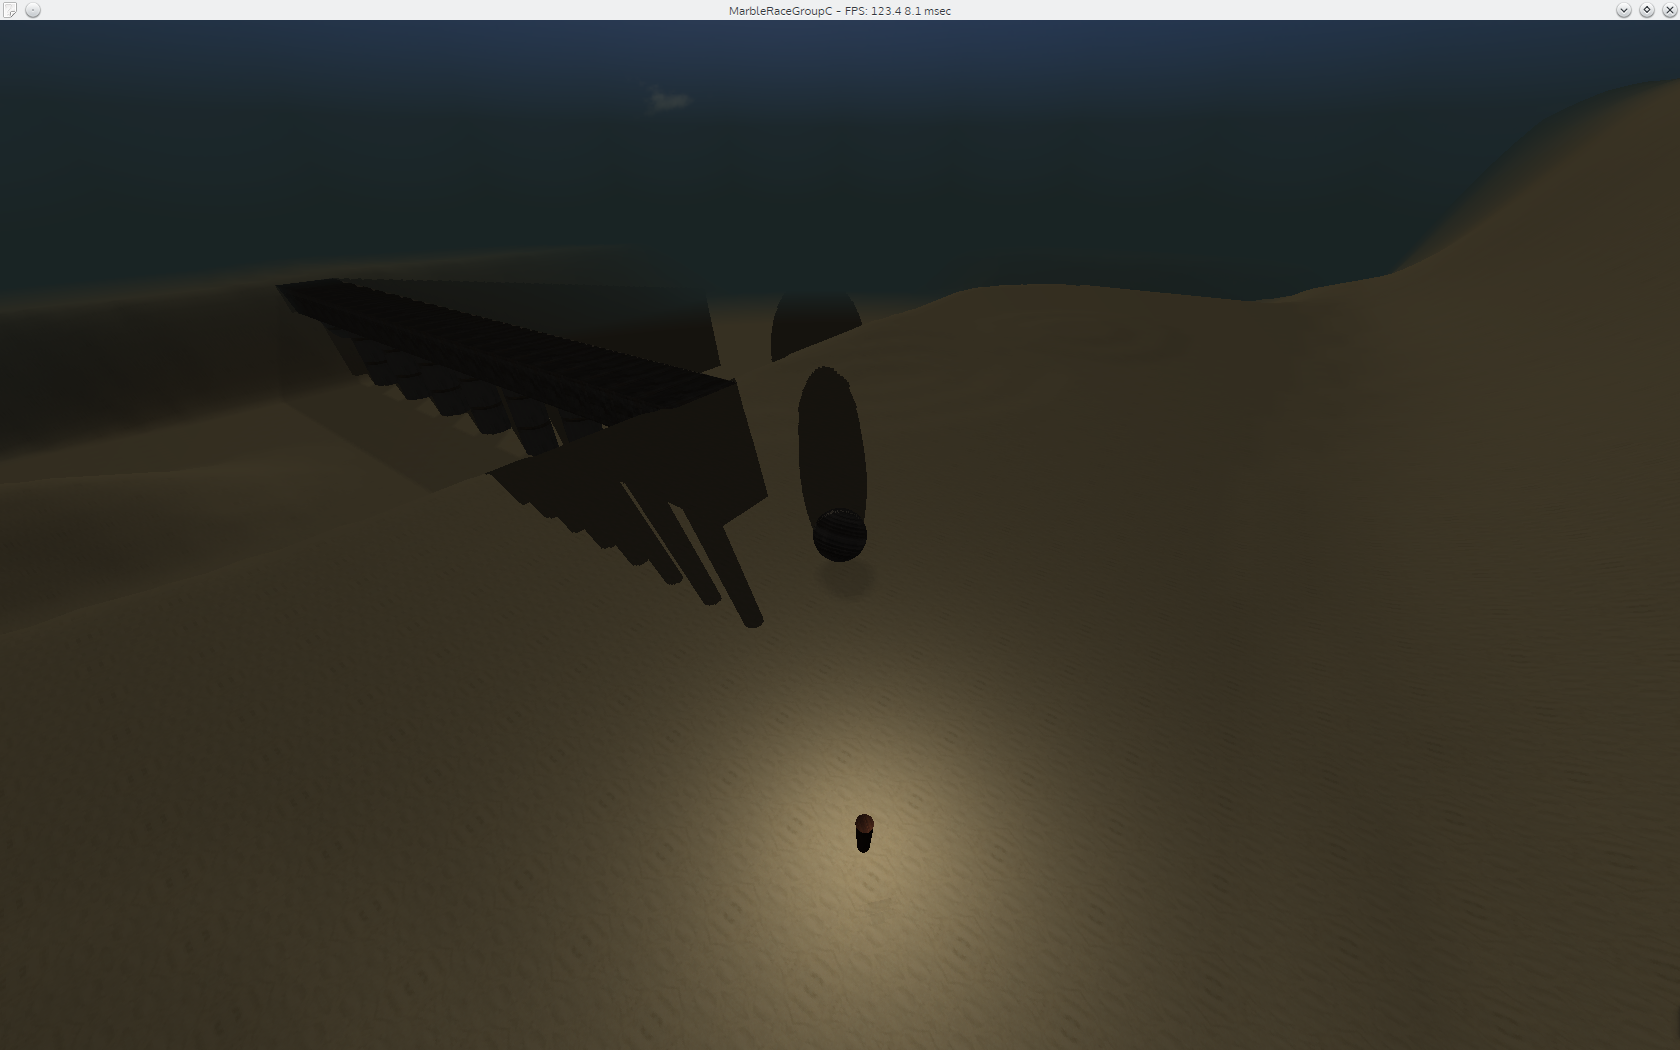
\includegraphics[width=11cm]{images/demo_m3}
\end{frame}

\end{document}
